
\documentclass{article}
\usepackage[left=2cm, right=2cm, top=2cm]{geometry}
\usepackage[utf8]{inputenc} 
\usepackage{graphicx} % to include images
\usepackage{amsmath} % For math mode
\usepackage{caption} % For captions
\usepackage{subcaption} % To use caption while using mini page
\usepackage{amssymb} % To use math symbols
\usepackage{multirow} %To combine multiple rows in a table
\usepackage[table]{xcolor} %To color rows / columns in table



%----------------------------MATLAB TEMPLATE -------------------------------------
\usepackage{listings}
\usepackage{color} %red, green, blue, yellow, cyan, magenta, black, white
\definecolor{mygreen}{RGB}{28,172,0} % color values Red, Green, Blue
\definecolor{mylilas}{RGB}{170,55,241}
%-----------------------------------------------------------------------------------------

\title{ECE 8540 Analysis of Tracking Systems \\ 
	Assignment 2}
\author{Vivek Koodli Udupa \\ C12768888}
\date{September - 11, 2018 }

\begin{document}

%Displaying Title
\begin{titlepage}
\maketitle
\pagenumbering{gobble}% Remove page numbers (and reset to 1)
\end{titlepage}
\pagenumbering{arabic}% Arabic page numbers (and reset to 1)

\section{Aim}
To derive and develop a nonlinear regression fit for the data set given using 'root finding' method. 

\section{Objectives}
\begin{enumerate}
	\item Plot the given data.
	\item Derive the equation for non-linear regression.
	\item Choose an initial value of 'a' and observe its effect on convergence.
	\item Find a suitable initial value for 'a' through trial and error method.
	\item Plotting the fit
\end{enumerate}
\section{Execution}
The given task is to fit a function of the form $y = ln(ax)$ where a is the unknown. The equation is non-linear in-terms of the unknown, a. To solve for non-linear terms, we use some variation of gradient decent. All these methods are iterative. They start with an initial approximation and then repeatedly  calculate the next guess based on the previous guess. Each of these successive approximations gets closer to the true solution. The iterations are typically stopped when the difference between two successive iterations are below certain threshold. This technique is known as \textbf{Non-linear regression.}

\subsection{Derivation}
\text{we know that,} 
\begin{align}
y &= ln(ax) \\
E &= \sum\limits_{i = 1}^N (y_i - ln(ax_i))^2 \\
\frac{\delta E}{\delta a} &= \sum\limits_{i = 1}^N [ 2(y_i - ln(ax_i)) (\frac{1}{a})] = 0 
\end{align}
After simplification ,we get  \\
\begin{align}
\frac{\delta E}{\delta a} &= \sum\limits_{i=1}^N (\frac{y_i - ln(ax_i)}{a}) \\
\therefore f(a) &=  \sum\limits_{i=1}^N (\frac{y_i - ln(ax_i)}{a}) \\
\end{align}
The derivative is 
\begin{align}
f'(a) &= \sum\limits_{i=1}^N [ \frac{a\frac{\delta}{\delta a}((ln(ax_i)) - (y_i - ln(ax_i))\frac{\delta}{\delta a}(a) }{ a^2 } ] \\
f'(a) &= \sum\limits_{i=1}^N [ \frac{ln(ax_i) - y_i - 1}{ a^2}]
\end{align}
Now we can find the value of a using the formula
\begin{align}
a_{n+1} &= a_n - \frac{f(a)}{f'(a)} 
\label{reg}
\end{align}
An initial guess of  'a' is taken and the next approximation '$a_{n+1}$'  is calculated using Equation \ref{reg}. Using the just obtained value, next approximation is calculated. This process is repeated till we converge to a desirable result.

\subsection{Plots and Observations}

\begin{figure}[h]
\centering
	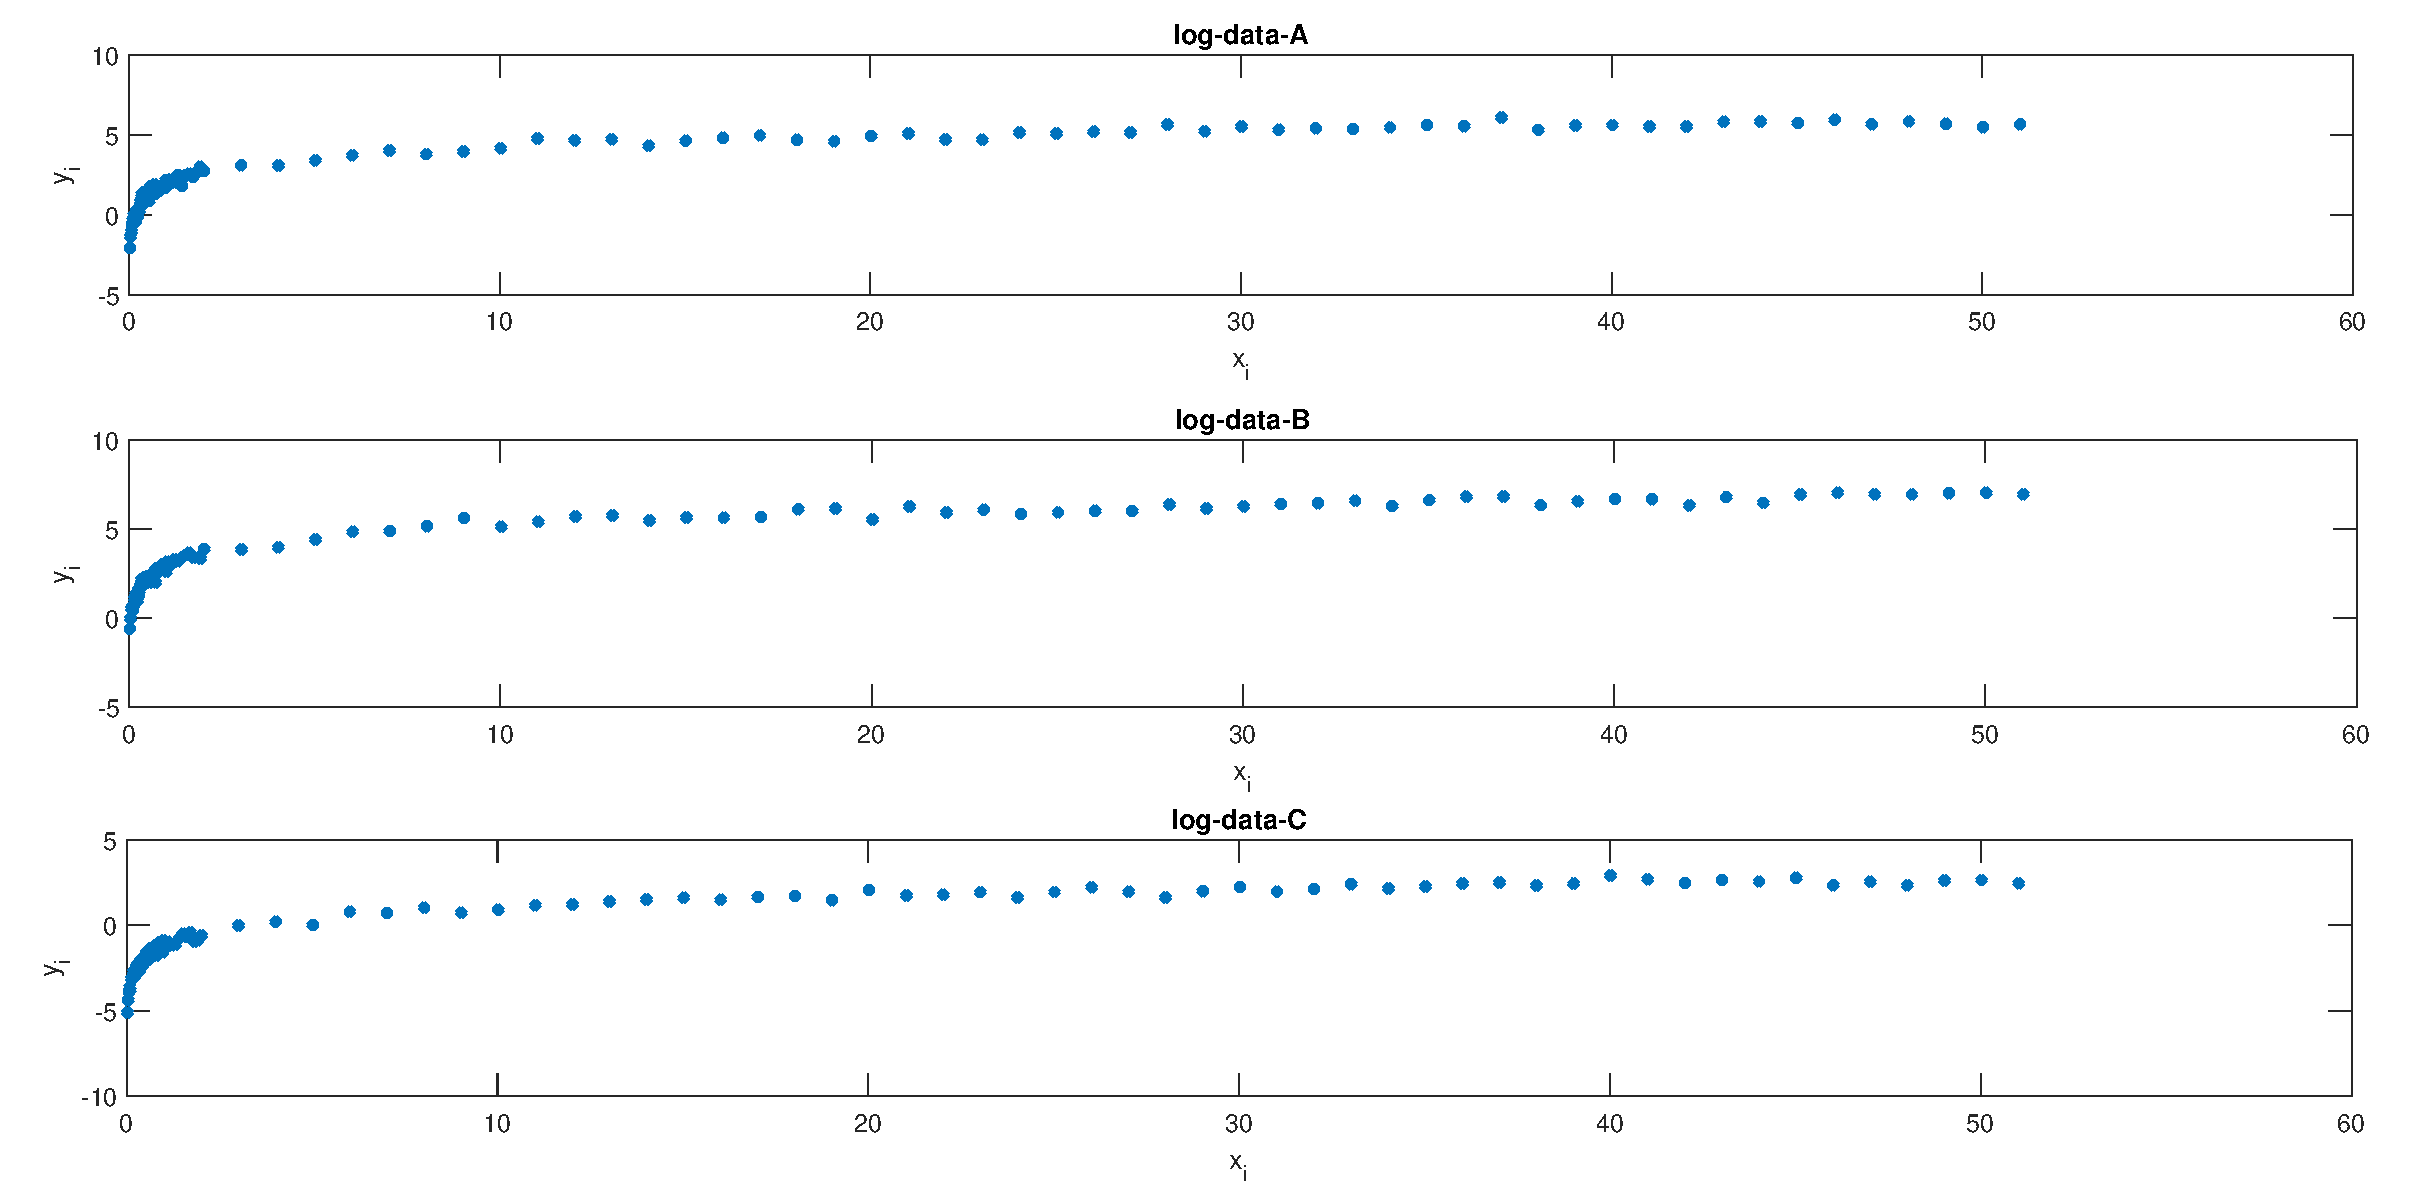
\includegraphics[width=\textwidth]{raw_data.eps}
	\caption{Raw Data plots}
	\label{fig:raw}
\end{figure}
\noindent
Figure \ref{fig:raw} is the plot of the raw data that was given.  We will use an equation if the form $y = ln(ax)$ to fit the above three data-sets.  \\

%Table one
\renewcommand{\arraystretch}{2} %changing row spacing to 2
\begin{table}[t]
\begin{center}
\begin{tabular}{ |c|c|c|c|c|c|}
\hline
Trials & Data set & Initial 'a' approximation & Final 'a' value & Iterations &MAX iterations \\
\hline 
%Trial 1
\multirow{3}{*}{1} & A  & 10 & 6.7114 & 7 & 500\\ \cline{2-6}
& B  & 10 & 18.9961 & 6 & 500 \\ \cline{2-6}
& C  & 10 & 9.9134e+152 & 500 & 500 \\
\hline
%Trial 2
\multirow{3}{*}{2} & A  & 5 & 6.7114 & 5 & 500\\ \cline{2-6}
& B  & 25 & 18.9961 & 6 & 500 \\ \cline{2-6}
& C  & 1 & 3.4673e+152 & 500 & 500 \\
\hline
%Trial 3
\rowcolor{green!10}
\multirow{3}{*}{3} & A  & 7 & 6.7114 & 4 & 500\\ \cline{2-6} \rowcolor{green!10} 
3& B  & 20 & 18.9961 & 4 & 500 \\  \cline{2-6} \rowcolor{green!10}
& C  & 0.1 & 0.2899 & 6 & 500 \\
%Trial 4
\multirow{3}{*}{4} & A  & 50 & 8.2663e+153 & 500 & 500\\ \cline{2-6}
& B  & 70 & 2.1240e+154 & 500 & 500 \\ \cline{2-6}
& C  & 100 & 6.6641e+153 & 500 & 500 \\
\hline
\end{tabular}
\end{center}
\caption{Observation of the effects of initial value on convergence}
\label{table:res}
\end{table}
\renewcommand{\arraystretch}{1} %changing it back to 1 otherwise every following table will have row spacing of 2

\noindent
Table \ref{table:res} shows the convergence of the system based on the initial approximation of a. Several trials were conducted with random initial values and Trial 3 looks like a satisfactory solution. \\
\\
Maximum of 500 iterations were set and the precision (i.e. $abs(a_{n+1} - a)$) set to  0.0001 \\
In Trial 1, the initial approximation was randomly chosen to be 10 for all the three data sets. Data set A converged to 6.7114, Data set B converged to 18.9961. They took 7 and 6 iterations respectively. Whereas Data-set C's calculation was finished by exceeding the MAX iteration and the final value of the unknown was found to be 9.9134e+152, which is very high. 
\newpage

\noindent
Figure \ref{fig:t1} through Figure \ref{fig:t4} shows the Non-linear fit drawn using the model $y=ln(ax)$ where a is the unknown , whose value is found is Table \ref{table:res}. Figure \ref{fig:t3} seems to be a good fit compared to the others. 

\begin{figure}
\centering
	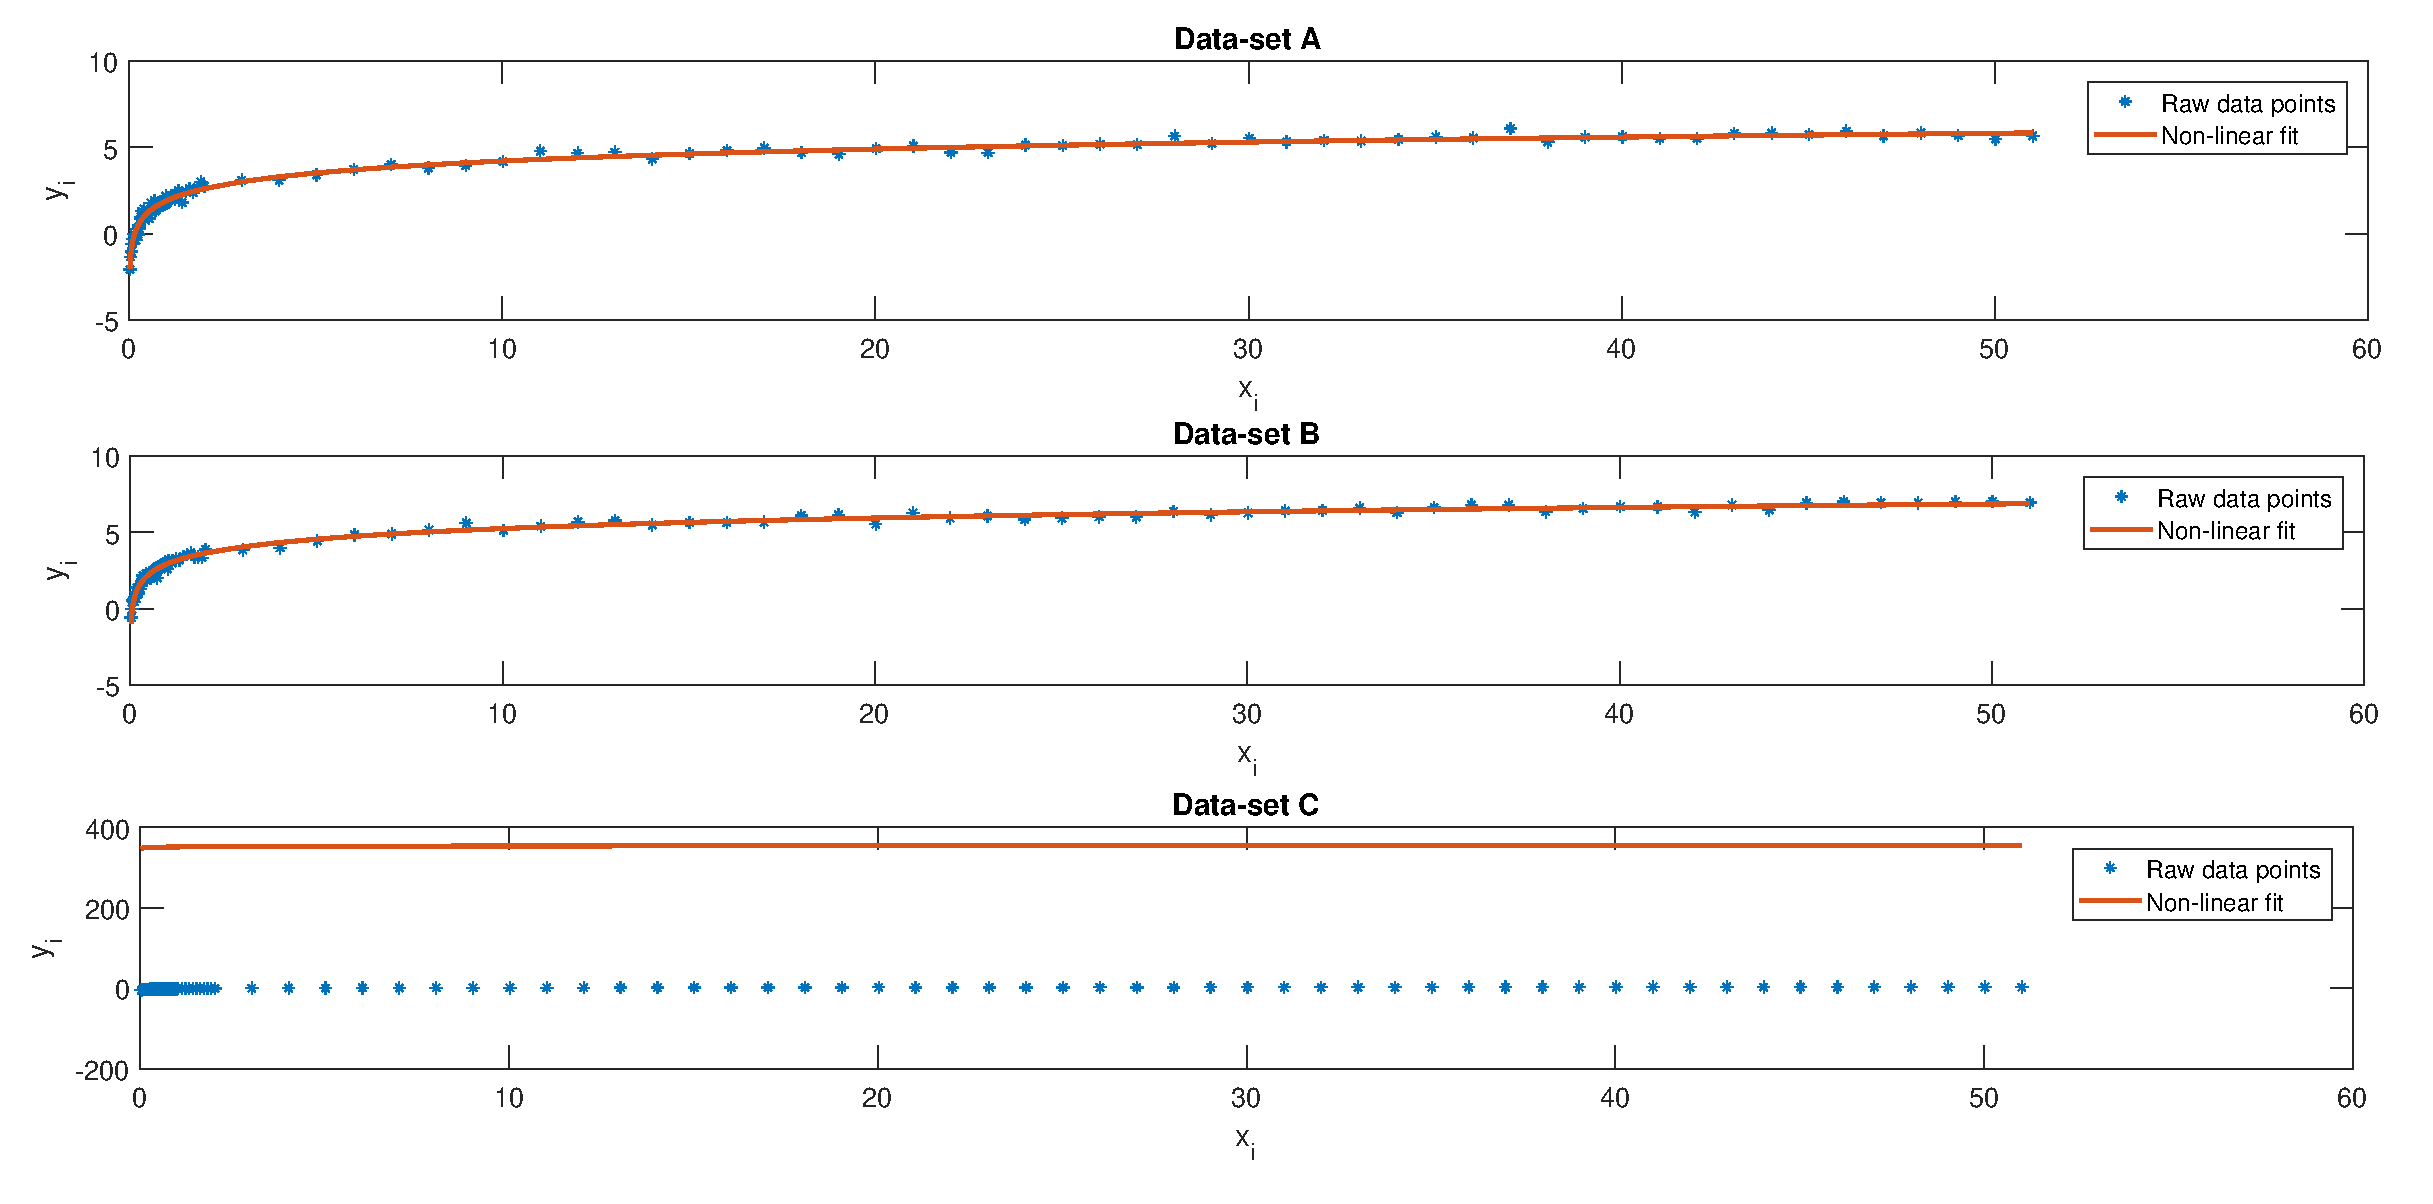
\includegraphics[width=\textwidth]{Trial2.eps}
	\caption{Non-linear fit using the value of unknown obtained in Trial 1}
	\label{fig:t1}
\end{figure}
\begin{figure}
\centering
	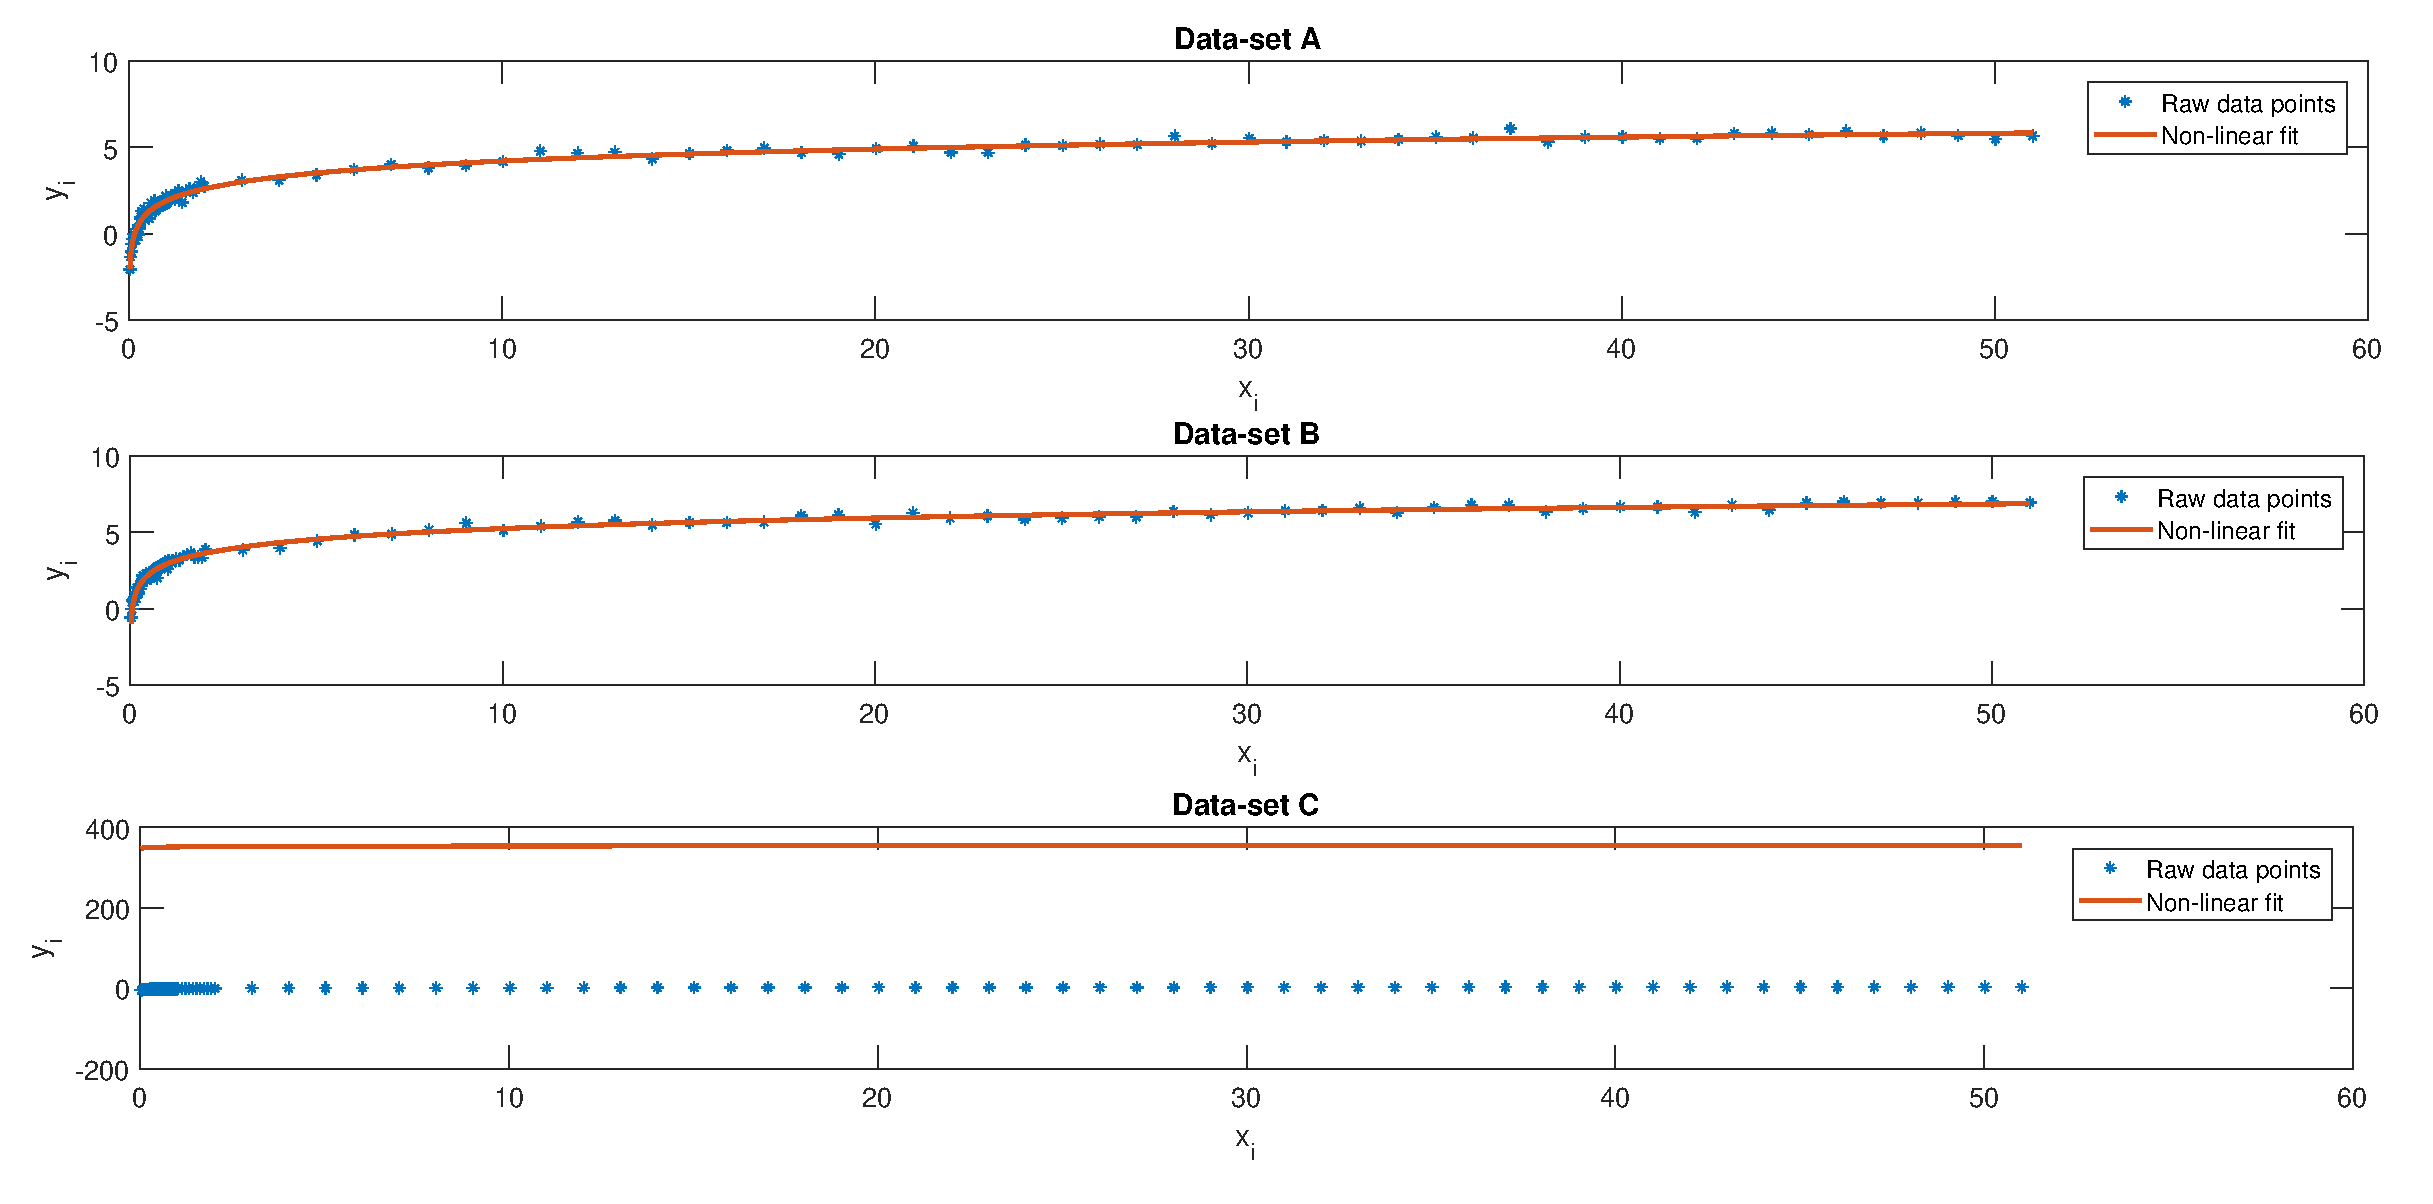
\includegraphics[width=\textwidth]{Trial2.eps}
	\caption{Non-linear fit using the value of unknown obtained in Trial 2}
	\label{fig:t2}
\end{figure}
\begin{figure}
\centering
	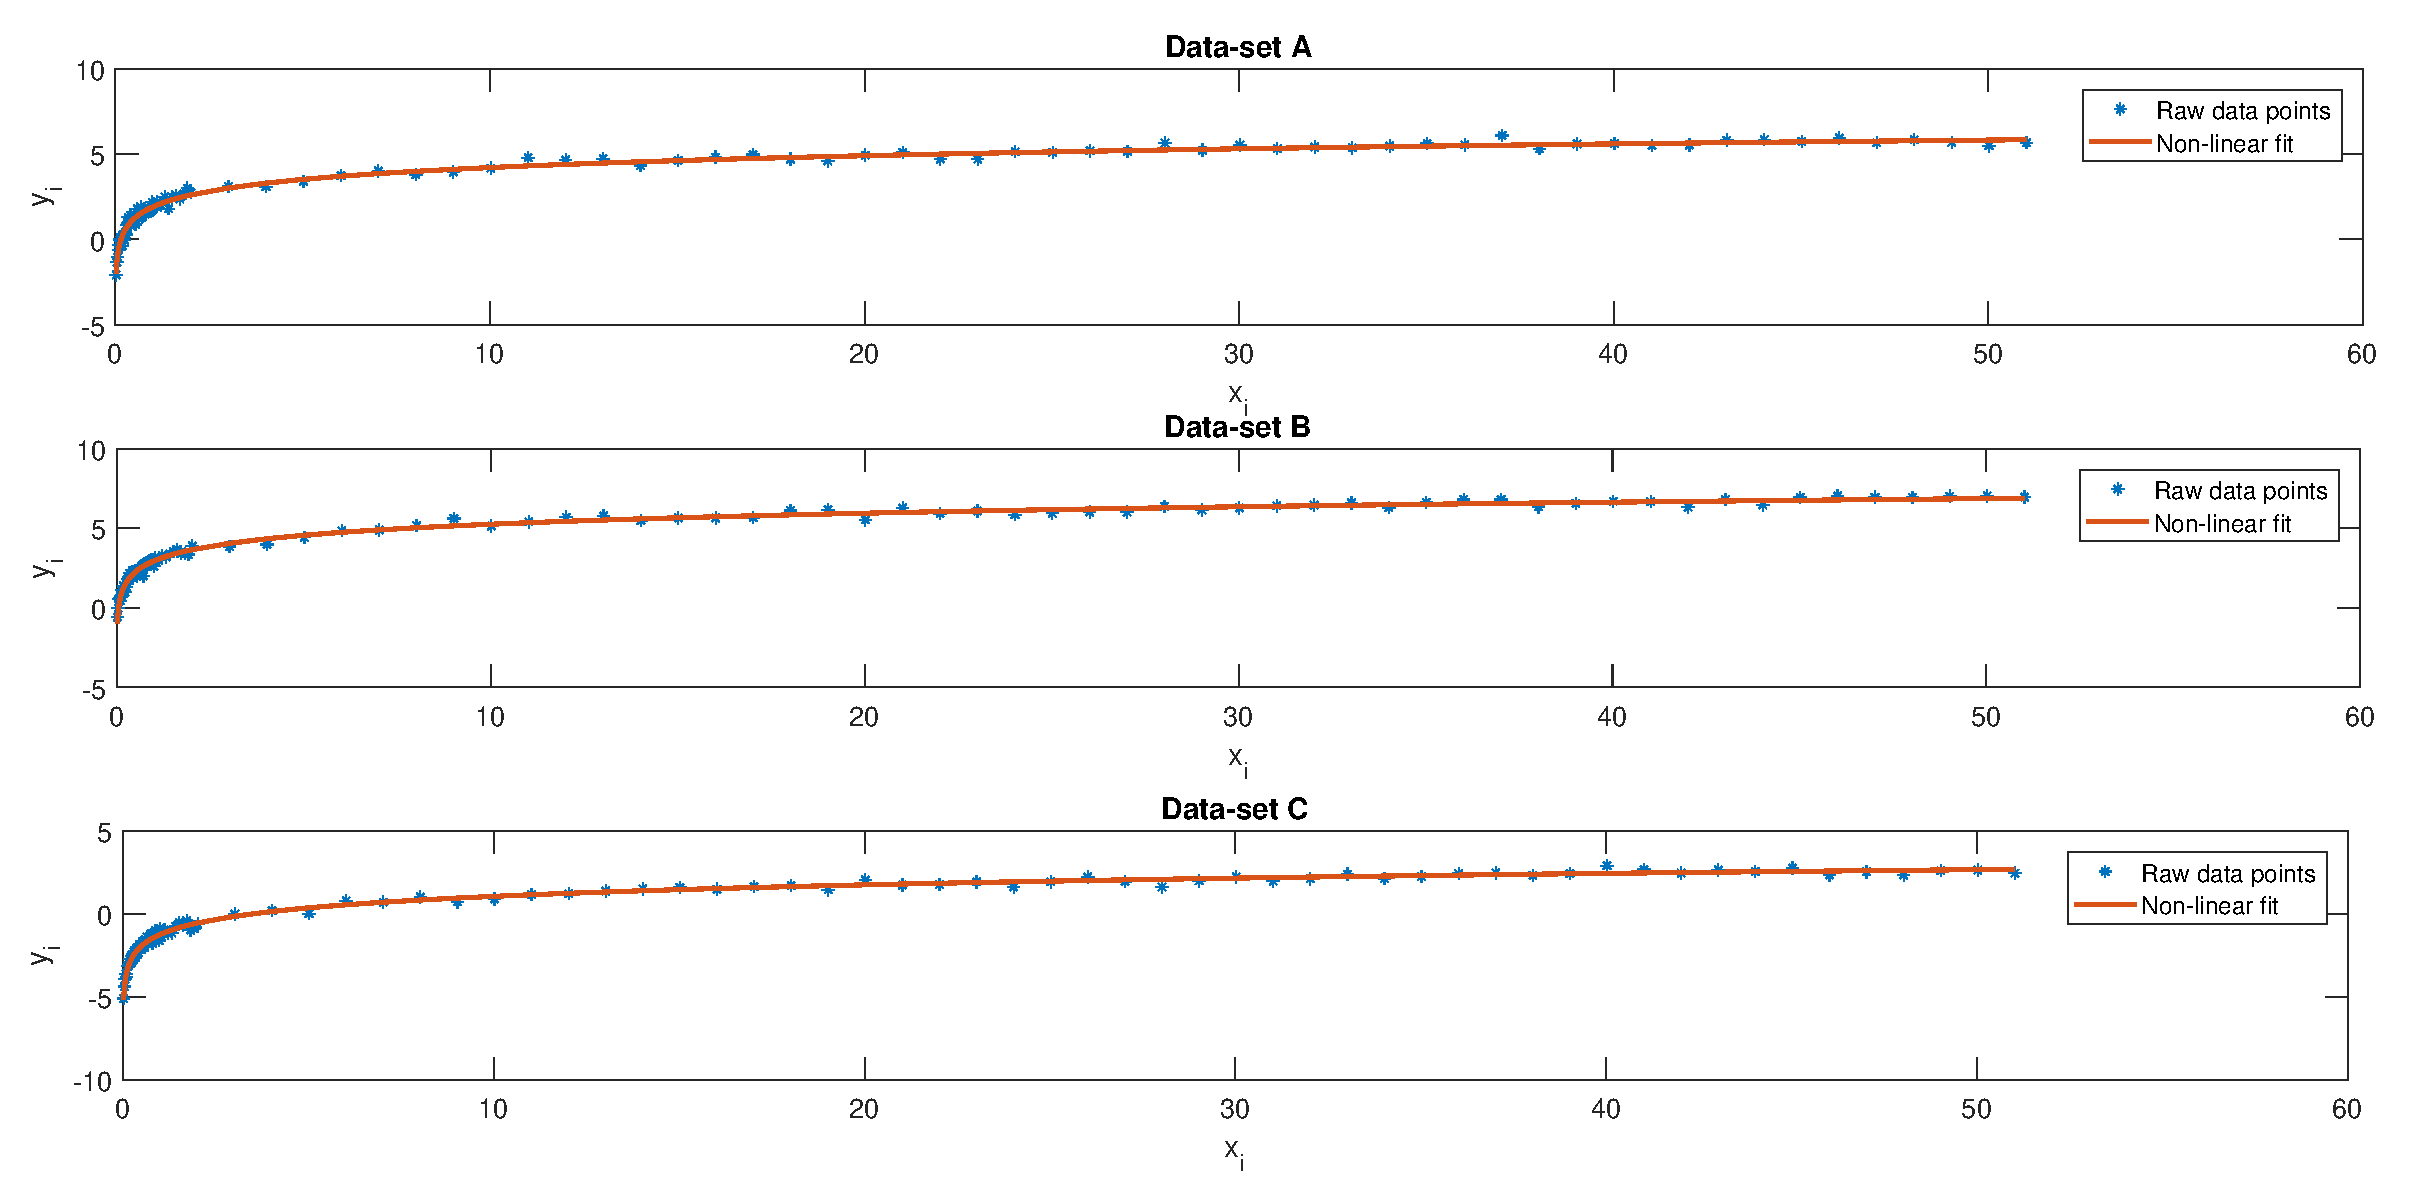
\includegraphics[width=\textwidth]{Trial3.eps}
	\caption{Non-linear fit using the value of unknown obtained in Trial 3}
	\label{fig:t3}
\end{figure}
\begin{figure}
\centering
	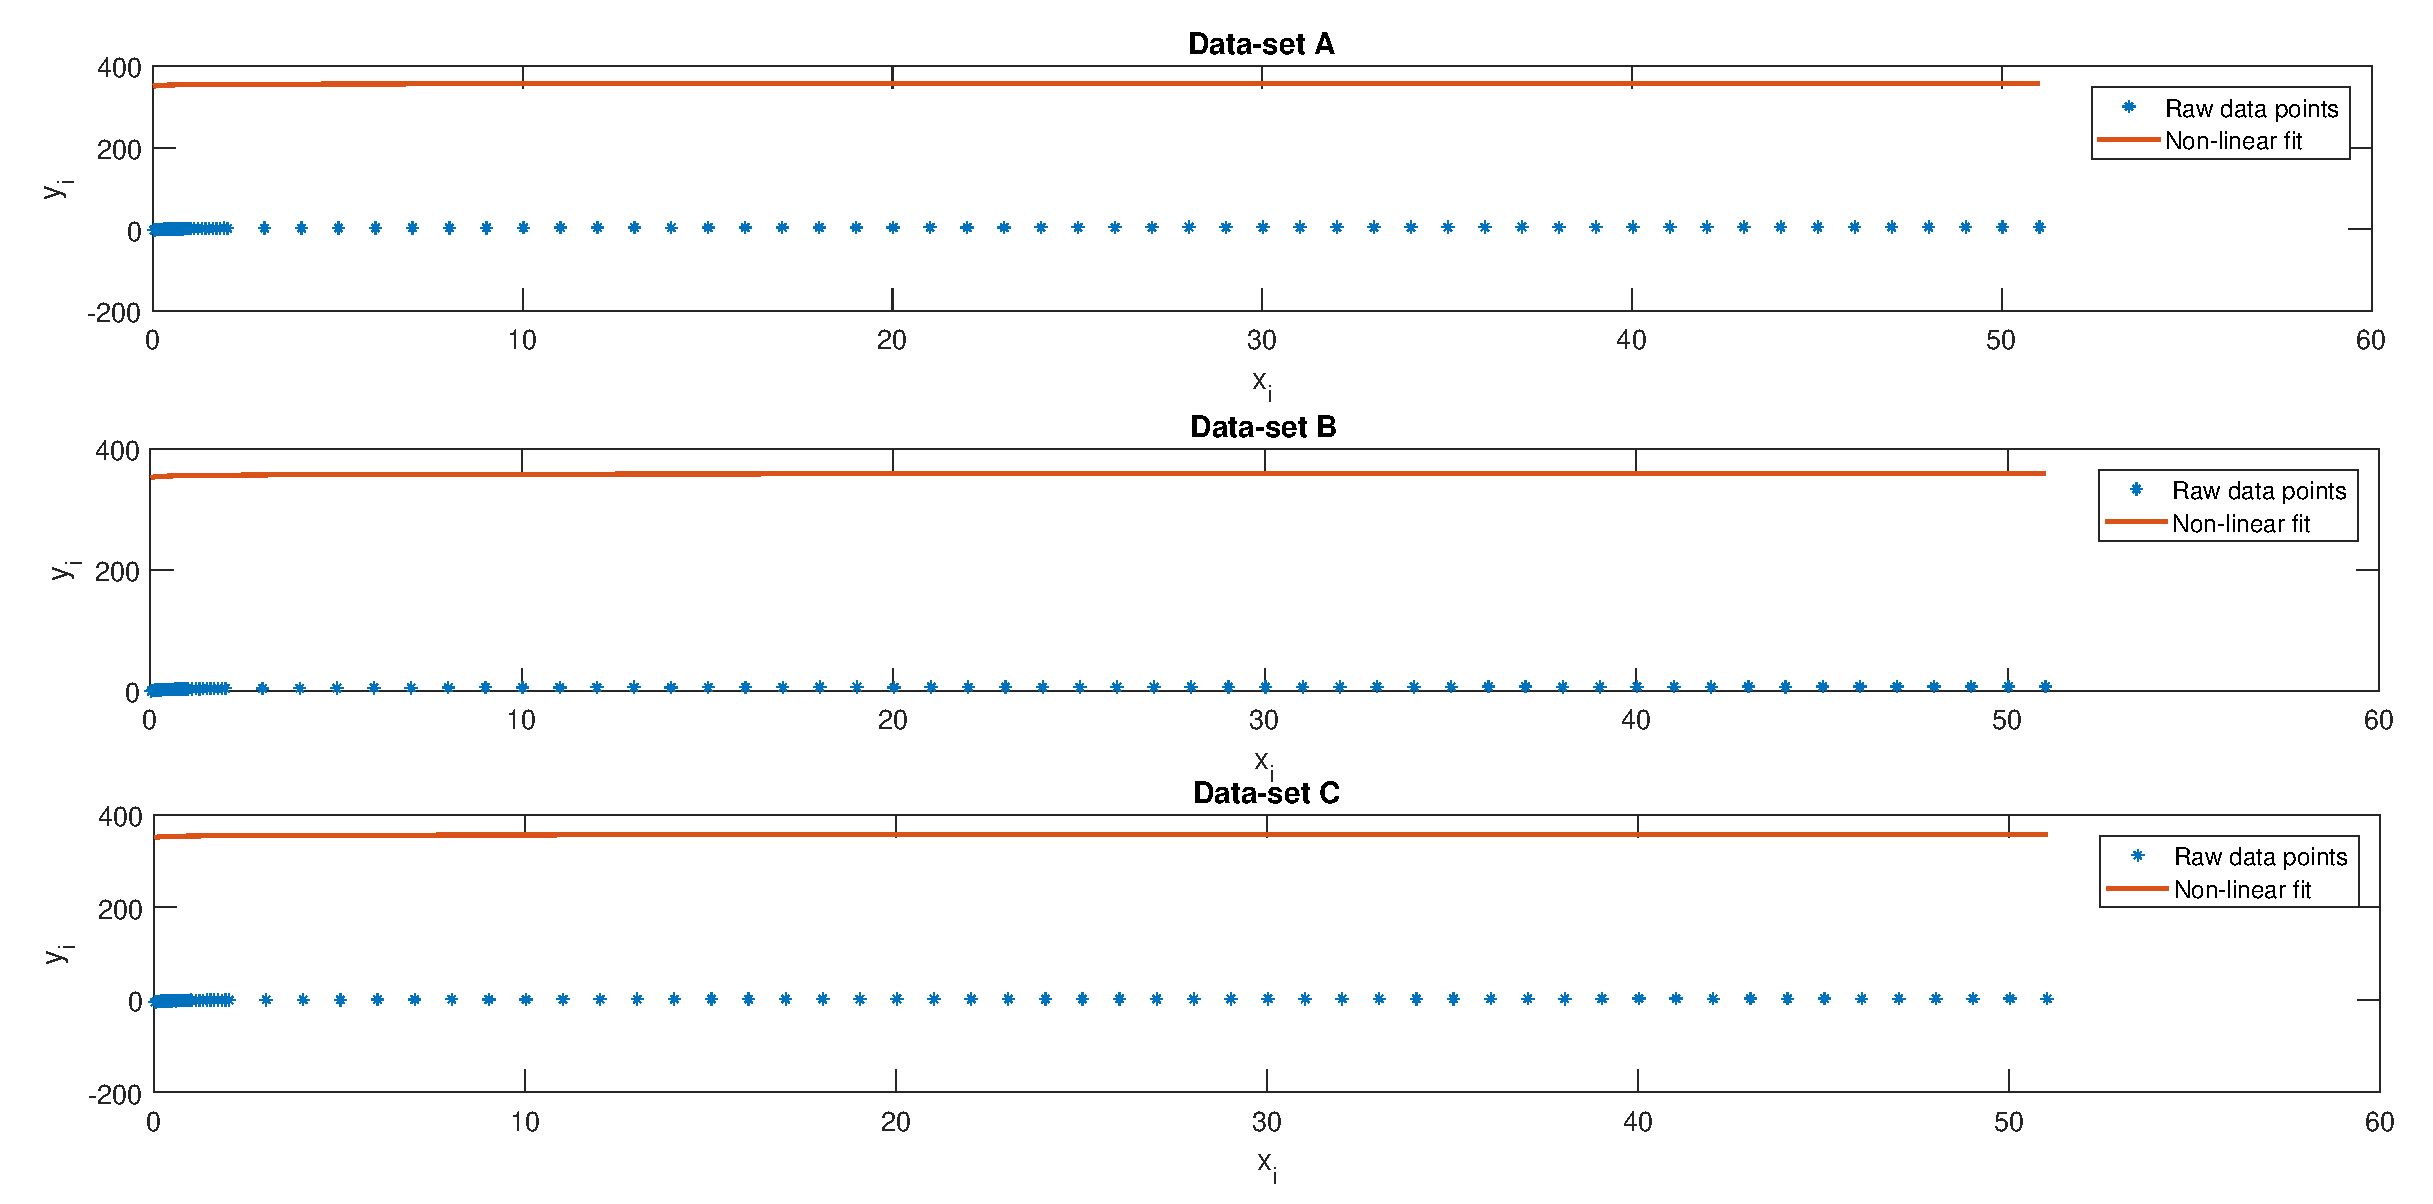
\includegraphics[width=\textwidth]{Trial4.eps}
	\caption{Non-linear fit using the value of unknown obtained in Trial 4}
	\label{fig:t4}
\end{figure}
\newpage
\section{Conclusion}
The Raw data points were plotted and a Non-linear model $y=ln(ax)$ was chosen for the fit. The values of the unknowns were calculated using the 'root finding' successive iteration method and the results are shown in Table \ref{table:res}. \\
\\
The value of the unknowns  for data-set A, B and C were found to be  \textbf{a1 = 6.7114}, \textbf{a2 = 18.9961} and \textbf{a3 = 0.2899} respectively. \\
\\
All the calculations were performed using MATLAB and the code is listed in the Appendix.

\newpage
%----------------------------------------------MATLAB LISTING TEMPLATE-------------------------

\lstset{language=Matlab,%
    %basicstyle=\color{red},
    breaklines=true,%
    morekeywords={matlab2tikz},
    keywordstyle=\color{blue},%
    morekeywords=[2]{1}, keywordstyle=[2]{\color{black}},
    identifierstyle=\color{black},%
    stringstyle=\color{mylilas},
    commentstyle=\color{mygreen},%
    showstringspaces=false,%without this there will be a symbol in the places where there is a space
    numbers=left,%
    numberstyle={\tiny \color{black}},% size of the numbers
    numbersep=9pt, % this defines how far the numbers are from the text
    emph=[1]{for,end,break},emphstyle=[1]\color{red}, %some words to emphasise
    %emph=[2]{word1,word2}, emphstyle=[2]{style},    
}


\section{Appendix}

\subsection{MATLAB Code}
\lstinputlisting{asg2.m}
\lstinputlisting{find_a.m}
%--------------------------------------------------------------------------------------------------------

\end{document}
